% ---------------------------------------------------------------------
% --- Arquivo principal e os demais serao os dos capitulos.
% --- EXPRESSÔES ENTRE <> DEVERÃO SER COMPLETADAS COM A INFORMAÇÂO ESPECÍFICA DO TRABALHO 
% ---------------------------------------------------------------------

\documentclass[ruledheader]{abnt_UFF}

%==\usepackage[colorlinks]{hyperref}
%\usepackage[printonlyused,withpage]{acronym}

%---pacotes para hiphenizacao e acentuacao em portugues
\usepackage[utf8]{inputenc}
\usepackage[brazil]{babel}
\usepackage[T1]{fontenc}


%---fornece a capacidade de criar hiperlinks no documento
%\usepackage[dvips,colorlinks=False, pdfstartview=FitV,citecolor=green,urlcolor=black,plainpages=false, pdftitle={Dissertação de Mestrado Yona Lopes}]{hyperref}%backref,
\usepackage[hidelinks, breaklinks, colorlinks=false, pdfstartview=FitV, linkcolor=black, citecolor=green,urlcolor=black,plainpages=false]{hyperref} % usar  hidelinks para esconder os links, continuara o link mas sem aparecer cor ou borda

\usepackage[breaklinks]{hyperref} % Problema quando o nome da figura/tabela/seção eh grande
%\usepackage[dvips,pdfstartview=FitV]{hyperref}%backref,
%\usepackage[dvips]{color}
	
%---pacotes para criacao de index
\usepackage{makeidx}
%\usepackage[pdftex,colorlinks=true, pdfstartview=FitV, linkcolor=black, citecolor=black,urlcolor=black,plainpages=false]{hyperref}
\usepackage{pdfcolmk}

%--- pacote para figuras
\usepackage{epsf}
\usepackage{epsfig,graphicx}
\usepackage{subfigure}


%--- pacote de simbolos
\usepackage{latexsym}
%\usepackage{textcomp}

%--- simbolos matematicos
\usepackage{amsmath}
%\usepackage{amssymb}

%----- códigos fonte
\usepackage{listings}
% opções do pacote listings
\lstset{numbers=left, language=java, stepnumber=1, firstnumber=1, numberstyle=\tiny, extendedchars=true, breaklines=true, frame=tb, basicstyle=\footnotesize, stringstyle=\ttfamily, showstringspaces=false backgroundcolor=\color{gray}}

\newcommand\JSONnumbervaluestyle{\color{blue}}
\newcommand\JSONstringvaluestyle{\color{red}}

% switch used as state variable
\newif\ifcolonfoundonthisline

\makeatletter

\lstdefinestyle{json}
{
	showstringspaces    = false,
	keywords            = {false,true},
	alsoletter          = 0123456789.,
	morestring          = [s]{"}{"},
	stringstyle         = \ifcolonfoundonthisline\JSONstringvaluestyle\fi,
	MoreSelectCharTable =%
	\lst@DefSaveDef{`:}\colon@json{\processColon@json},
	basicstyle          = \ttfamily,
	keywordstyle        = \ttfamily\bfseries,
}

% flip the switch if a colon is found in Pmode
\newcommand\processColon@json{%
	\colon@json%
	\ifnum\lst@mode=\lst@Pmode%
	\global\colonfoundonthislinetrue%
	\fi
}

\lst@AddToHook{Output}{%
	\ifcolonfoundonthisline%
	\ifnum\lst@mode=\lst@Pmode%
	\def\lst@thestyle{\JSONnumbervaluestyle}%
	\fi
	\fi
	%override by keyword style if a keyword is detected!
	\lsthk@DetectKeywords% 
}

% reset the switch at the end of line
\lst@AddToHook{EOL}%
{\global\colonfoundonthislinefalse}

\makeatother

% pacote para posicionamento de tabelas e figuras
\usepackage{float}
\restylefloat{table}


%--- pacote para gerar pseudo-codigo
%\usepackage{algorithm}
%\usepackage{algorithmic}
% \usepackage[linesnumbered,boxed,lined]{algorithm2e} 
\usepackage[algoruled,portuguese,linesnumbered]{algorithm2e} 
%\floatname{algorithm}{Algoritmo}

%--- outros pacotes
\usepackage{url}
\usepackage{longtable}
\usepackage{lscape}

%\usepackage[notbib, notlof, notlot]{tocbibind}

%Tabela Colorida e pacotes de tabela
%\usepackage{colortbl}
\usepackage{array}

%--- Acronyms
%\usepackage{acronym}
\usepackage[printonlyused,withpage]{acronym}

\usepackage{multicol}
\usepackage{multirow}
\usepackage{rotating}

%--- Notes
\usepackage{todonotes}

\hyphenation{
a-de-qua-da-men-te 
di-men-sio-na-men-to 
re-di-re-cio-na
}

%---------usando tipo de fonte padrao
\renewcommand{\ABNTchapterfont}{\bfseries\fontfamily{cmr}\fontseries{b}\selectfont}
\renewcommand{\ABNTsectionfont}{\bfseries\fontfamily{cmr}}

\newcommand{\todot}[1]{\todo[color=green!40,fancyline]{#1}}


\makeindex
% --- -----------------------------------------------------------------
% --- Documento Principal.
% --- -----------------------------------------------------------------
%\usepackage[pdftex]{hyperref}
%\hypersetup{colorlinks, sitecolor=black, pdftex}
\begin{document}

% --- -----------------------------------------------------------------
% --- Titulo, abstract, dedicatorias e agradecimentos.
% --- Indice geral, lista de figuras e tabelas.
% --- -----------------------------------------------------------------

% --- -----------------------------------------------------------------
% --- Elementos usados na Capa e na Folha de Rosto.
% --- EXPRESSES ENTRE <> DEVERO SER COMPLETADAS COM A INFORMAO ESPECFICA DO TRABALHO
% --- E OS SMBOLOS <> DEVEM SER RETIRADOS 
% --- -----------------------------------------------------------------
\autor{NICOLAS DE SOUSA TEODOSIO E VICTOR HUGO NOVAIS RODRIGUES} % deve ser escrito em maiusculo

\titulo{ANÁLISE DE SENTIMENTO E MINERAÇÃO DE OPINIÕES APLICADO NO TWITTER} % deve ser escrito em maiusculo

\instituicao{INSTITUTO INFNET} % deve ser escrito em maiusculo

\orientador{CASSIUS FIGUEIREDO}% deve ser escrito em maiusculo - preencher com o nome do seu orientador

%\coorientador{NOME} %preencher se houver.

\local{RIO DE JANEIRO} % deve ser escrito em maiusculo

\data{2016} % ano da defesa

\comentario{Trabalho de Conclusão de Curso apresentado ao Programa de Graduação em Engenharia da Computação do \mbox{Instituto Infnet} como parte dos requisitos necessários à obtenção do título de \mbox{Bacharel em Engenharia da Computação}.}%preencha com a sua area de concentracao


% --- -----------------------------------------------------------------
% --- Capa. (Capa externa, aquela com as letrinhas douradas)(Obrigatorio)
% --- ----------------------------------------------------------------
\capa

% --- -----------------------------------------------------------------
% --- Folha de rosto. (Obrigatorio)
% --- ----------------------------------------------------------------
\folhaderosto


\pagestyle{ruledheader}
\setcounter{page}{1}
\pagenumbering{roman}

% --- -----------------------------------------------------------------
% --- Ficha Catalográfica. (Obrigatorio)
% --- ----------------------------------------------------------------
%
%\cleardoublepage
%\thispagestyle{empty}
%\vspace*{130mm}
%
%\begin{flushright}
%
%\hspace{8em}
%\fbox{\begin{minipage}{10cm}

%....

%\end{minipage}}
%
%\end{flushright}
%\newpage

% --- -----------------------------------------------------------------
% --- Termo de aprovacao. (Obrigatorio)
% --- ----------------------------------------------------------------


\cleardoublepage
\thispagestyle{empty}

\vspace{-60mm}

\begin{center}
   {\large NICOLAS DE SOUSA TEODOSIO E VICTOR HUGO NOVAIS RODRIGUES}\\
   \vspace{7mm}

  PySent: ANÁLISE DE SENTIMENTO E MINERAÇÃO DE DADOS APLICADO NO TWITTER\\
%   \vspace{10mm}
 \vspace{8mm}  %diminui para ajustar a data que estava pulando para outra folha
\end{center}

\noindent
\begin{flushright}
\begin{minipage}[t]{8cm} 
%\begin{minipage}{\columnwidth}

Trabalho de Conclusão de Curso apresentado ao Programa de Graduação em Engenharia da Computação do \mbox{Instituto Infnet} como parte dos requisitos
necessários à obtenção do título de \mbox{Bacharel em Engenharia da Computação}

\end{minipage}
\end{flushright}
\vspace{ 5mm}  %original 1cm
\noindent
Aprovada em XX agosto de 2016. \\
\begin{flushright}
  \parbox{15cm}
  {
  \begin{center}
  BANCA EXAMINADORA \\
  \vspace{5mm}
  \rule{11cm}{.1mm} \\
	Prof. Cassius Figueiredo, M.Sc. - Orientador \\ 
	Instituto INFNET \\
  \vspace{5mm}
  \rule{11cm}{.1mm} \\
    A definir \\ 
  \vspace{5mm}
  \rule{11cm}{.1mm} \\
    A definir \\ 
  \end{center}
  }
\end{flushright}
\begin{center}
  \vspace{4mm} % 
 Rio de Janeiro \\
  %\vspace{6mm}
  2016
\end{center}

% --- -----------------------------------------------------------------
% --- Dedicatoria.(Opcional)
% --- -----------------------------------------------------------------
\cleardoublepage
\thispagestyle{empty}
\vspace*{200mm}

\begin{flushright}
{\em 
Às nossas famílias e amigos que durante esses cinco anos nos apoiaram nos momentos mais difíceis.
Aos colegas e mestres que nos acompanharam nesta empreitada que no início eram desconhecidos, e hoje amigos que levaremos para o resto da vida.
%Dedicatória(s): À blá blá%Elemento opcional onde o autor presta homenagem ou dedica seu trabalho (ABNT, 2005).
}
\end{flushright}
\newpage


% --- -----------------------------------------------------------------
% --- Agradecimentos.(Opcional)
% --- -----------------------------------------------------------------
\pretextualchapter{Agradecimentos}
\hspace{5mm}
Agradecemos inicialmente ao professor Cassius Figueiredo pelo total suporte nesse trabalho e por seu papel fundamental na nossa trajetória como alunos de Engenharia da Computação. Aos nossos pais, Rosângela de Sousa Teodosio, José Carlos Teodosio da Silva, Deise Luci Gouveia Novais e Paulo Roberto Rodrigues que nos proporcionaram uma base com valores familiares que nos permitiram seguir sempre nossos estudos, independentemente das dificuldades que surgiram pelo caminho.

Aos colegas de classe que fizemos durante estes 5 anos. Esperamos que, de uma forma ou de outra, todos alcancem o que desejam se seguirem o caminho do trabalho duro e da perseverança.

Aos amigos que nos ajudaram profissionalmente e academicamente, servindo de exemplo e dando conselhos que nos tornaram os profissionais que hoje somos: Ezequiel Bertti, João Leite, Thúlio Costa, Felipe Salvini, Dalton Matos, Alan Dieguez, Jesue Sousa e Cesar Frias.

Eu, Nicolas, agradeço à minha esposa Joyce Kelly Dias da Costa e minha irmã Jéssica de Sousa Teodosio por estar ao meu lado durante todo o curso e suportar todos os percalços que enfrentei até aqui.

Eu, Victor Hugo Novais Rodrigues, agradeço ao meu avô e grande exemplo de força, Manuel Ferreira Novais. Aos padrinhos Mauro Sérgio de Almeida Rubianes, Maysa Alexandrino dos Santos Rubianes e Maria Dionísia Pimentel dos Santos e aos tios Manoel de Carvalho Almeida e Vania Luci Gouveia Novais Almeida por todo carinho e apoio na minha criação e educação. À minha namorada Thays Scapin Coca pelo companheirismo e amor que me permitiram ir mais longe do que eu jamais sonhei.

Um agradecimento especial aos professores que cruzaram nossos caminhos durante o curso sempre transmitindo o conhecimento, experiência e sabedoria da maneira mais nobre possível.

Pedimos desculpas àqueles que porventura tenham sido esquecidos. Esta graduação foi fruto do esforço de muitos e não só das duas pessoas que o encabeçam.
% --- -----------------------------------------------------------------
% --- Resumo em portugues.(Obrigatorio)
% --- -----------------------------------------------------------------
\begin{resumo}

Atualmente a internet e micro blogs em geral têm se tornado uma ferramenta de comunicação poderosa entre seus usuários. Bilhões de pessoas compartilham informações e opiniões a todo momento, fazendo desse espaço um ótimo campo de pesquisas comerciais, acadêmicas e sociológicas.  Como esse fenômeno é relativamente recente, as pesquisas destinadas ao tema são consideradas novas, o Twitter, por exemplo foi criado apenas em 2006 e hoje possui 310 milhões de usuários ativos por mês .


Os principais desafios para aplicação da análise de sentimento estão relacionados a linguagens naturais sensíveis ao contexto, que não trazem resultados satisfatórios quando utilizam-se modelos matemáticos muito simples, sendo necessário um grande investimento de tempo em aperfeiçoar os modelos matemáticos disponíveis e adaptá-los à solução em questão.


O objetivo deste trabalho é explorar o potencial existente em pesquisas de opinião,  que podem ser feitas através de análises nas comunicações utilizando a  língua portuguesa nas redes sociais todos os dias, mostrando que o conteúdo escrito pelos usuários tem uma importância tão grande quanto a de números exibidos em redes sociais. A prática desse trabalho demandou uso de algoritmos matemáticos mais elaborados, aquisição de bases de palavras para o uso desse algoritmo, aplicação de um processo produtor-consumidor e acesso ao Twitter para coleta de dados. Foi realizada uma análise de caso sobre o Oscar 2016 para validar a efetividade desse trabalho. 


O algoritmo utilizado foi o \textit{Naive Bayes}, um algoritmo probabilístico, que realiza a análise de sentimento do oscar no momento de picos do evento, um deles sendo a premiação de melhor ator, atriz e filme. Nesses picos foram feitas análises de quantidade  e  taxa de polaridade. Seus resultados atestam a possibilidade da língua portuguesa como objeto de análise para a mineração de dados de forma relevante.


{\hspace{-8mm} \bf{Palavras-chave}}: Análise de sentimento, mídias sociais, twitter, mineração de opiniões, processamento de linguagem natural, linguagens sensíveis a contexto, naive bayes.

%redefine todas siglas para não usado
\acresetall

\end{resumo}

% --- -----------------------------------------------------------------
% --- Resumo em lingua estrangeira.(Obrigatorio)
% --- -----------------------------------------------------------------
\begin{abstract}
	
Today the internet and micro blogs in general have become a powerful communication tool among its users. Billions of people share information and opinions at all times, making this space a great field of commercial, academic and sociological research. As this phenomenon is relatively recent, research aimed at the topic is considered new, Twitter, for example was created only in 2006 and today has 310 million active users per month.


The main challenges for the application of the feeling analysis are related to context-sensitive natural languages, which do not yield satisfactory results when very simple mathematical models are used, requiring a great investment of time in improving the mathematical models available and adapting them to the solution in question.


The objective of this work is to explore the potential of opinion polls, which can be done through analysis in the communications using the Portuguese language in social networks every day, showing that the content written by users is as important as that of numbers displayed on social networks. The practice of this work required the use of more elaborate mathematical algorithms, acquisition of word bases for the use of this algorithm, application of a producer-consumer process and access to Twitter for data collection. A case study on the Oscar 2016 was conducted to validate the effectiveness of this work.


The algorithm used was the Naive Bayes, a probabilistic algorithm that performs the sentiment analysis of oscar at the moment of the peaks of the event, one of them being the best actor, actress and film award. At these peaks were made analyzes of quantity and polarity rate. Their results attest to the possibility of the Portuguese language as an object of analysis for data mining in a relevant way.	


{\hspace{-8mm} \bf{Palavras-chave}}: Sentiment analisys, social midia, twitter, opnion mining, natural language process, Context-sensitive languages, naive bayes.


%redefine todas siglas para não usado
\acresetall

\end{abstract}

% --- -----------------------------------------------------------------
% --- Lista de figuras.(Opcional)
% --- -----------------------------------------------------------------
\cleardoublepage
\listoffigures
\label{listafiguras}
\acresetall

% --- -----------------------------------------------------------------
% --- Lista de tabelas.(Opcional)
% --- -----------------------------------------------------------------
\cleardoublepage
\label{listatabelas}
\listoftables
\cleardoublepage
\acresetall

% --- -----------------------------------------------------------------
% --- Lista de abreviatura.(Opcional)
%Elemento opcional, que consiste na relação alfabética das abreviaturas e siglas utilizadas no texto, seguidas das %palavras ou expressões correspondentes grafadas por extenso. Recomenda-se a elaboração de lista própria para cada %tipo (ABNT, 2005).
% --- ----------------------------------------------------------------
\cleardoublepage
\pretextualchapter{Lista de Abreviaturas e Siglas}
\begin{acronym}
	\acro{API}{Application Program Interface}
	\acro{PLN}{Processamento de Linguagem Natural}
	\acro{IA}{Inteligência Artificial}
	\acro{REST}{\textit{Representational state transfer}}
	\acro{SOAP}{\textit{Simple Object Access Protocol}}
	\acro{JSON}{\textit{Javascript Object Notation}}
	\acro{WSDL}{\textit{Web Services Description Language}}
	\acro{HTTP}{\textit{Hipertext Transfer Protocol}}
	\acro{XML}{\textit{Extensible Markup Language}}
	\acro{FIFO}{\textit{First-In-First-Out}}
	\acro{NLTK}{\textit{\textit{Natural Language Toolkit}}}
	\acro{SQL}{\textit{Structure Query Language}}
	\acro{NoSQL}{\textit{Non Structure Query Language}}
	\acro{RDBMS}{\textit{Relational database management system}} 
	
\end{acronym}

% --- -----------------------------------------------------------------
% --- Sumario.(Obrigatorio)
% --- -----------------------------------------------------------------
\pagestyle{ruledheader}
\tableofcontents
\acresetall



% --- -----------------------------------------------------------------
% --- Insercao dos capitulos.
% --- -----------------------------------------------------------------
\pagestyle{ruledheader}
\setcounter{page}{1}
\pagenumbering{arabic}

\inputencoding{utf8}

\chapter{Introdução} \label{cap:1}

Através do fenômeno da popularização da Internet vivemos hoje um período conhecido como "Era da conhecimento" \cite{lastres1999informaccao}.
Nesse contexto, redes sociais conhecidas, como Facebook e Twitter se tornaram bastante populares por permitirem a seus usuários acesso à um ambiente onde todos possuem voz e vez para se expressar e por consequência, para se informar sobre tudo que acontece no mundo.
Através de \ac{API} disponibilizadas por essas redes sociais, possuímos fácil acesso à um grande volume de opiniões catalogadas - através de \textit{hashtags} - que podem ser utilizadas em pesquisas de opinião sobre um tema ou assunto específico. Tal cenário apresenta-se como uma grande oportunidade de pesquisa em áreas acadêmicas, sociais e comerciais.
Porém, quando o objeto de estudo é a língua portuguesa, nota-se que a mesma carece de trabalhos e implementações na área de mineração de opiniões e análise de sentimento (REFERÊNCIA). Alguns motivos explicam essa carência: poucos investimentos na área de ciência e engenharia da computação em nosso país e a grande dificuldade que a língua portuguesa apresenta ao ser interpretada através de processamento de linguagem natural. \cite{santos2000projecto}


\section{Motivação e Objetivos}\label{sec:1_inicio}
%A motivação deste trabalho é explorar o potencial contido no conteúdo digital gerado todos os dias em redes sociais por %usuários brasileiros. Tais dados possuem informações valiosas que podem ser explorados de inúmeras maneiras



\section{Principais contribuições}\label{sec:1_principais_contribuicoes}

\section{Recursos utilizados}\label{sec:1_recursos_utilizados}

\section{Organização do trabalho}\label{sec:1_org}

Este trabalho está estruturado em 5 capítulos da seguinte forma: no Capítulo~\ref{cap:referencial_teorico}, para embasamento teórico, são apresentados os conceitos de (CONTINUA). Em seguida, no Capítulo~\ref{cap:proposta} , é feita uma análise sobre os principais trabalhos relacionados ao uso dos ... . No Capítulo~\ref{cap:referencial_teorico}, os conceitos do arcabouço utilizado ... , são descritos. Nesse capítulo são mostrados os motivos para a escolha desse arcabouço, .... A proposta XXX é apresentada no Capitulo~\ref{cap:proposta}, onde a arquitetura da proposta é detalhada, assim como seus componentes e algoritmos. Em seguida, o Capítulo~\ref{cap:resultados} apresenta as ferramentas utilizadas para implementação da proposta, o ambiente implementação, a descrição dos experimentos e os principais resultados obtidos com o XXX, assim como a análise dos valores encontrados. Por fim, o Capítulo~\ref{cap:conc} conclui este trabalho, ressaltando os objetivos alcançados com as propostas. As principais vantagens e desvantagens da proposta são discutidas, assim como alguns trabalhos futuros que podem ser desenvolvidos. 

\chapter{Referencial Teórico}\label{cap:referencial_teorico}

\section{Mineração de opinião}\label{sec:mineracao_dados}

É de conhecimento comum que há um acúmulo de dados por toda a internet. Artigos, informações de usuários, comportamento de usuários, essas são alguns tipos de informação que pode ser encontrada hoje na internet. Esse grande acumulo não garante informações confiáveis ou uma análise correta sobre os dados, por isso hoje há uma grande urgência para novas teorias computacionais e ferramentas que ajudem a analisar essa quantidade de dados que só aumenta \cite{fayyad1996data}. E dentro dessa enorme gama de dados, existem as informações adicionadas por usuários através de texto que remetem a suas reações a determinadas situações ou objetos.

\begin{figure}[ht]
	\centering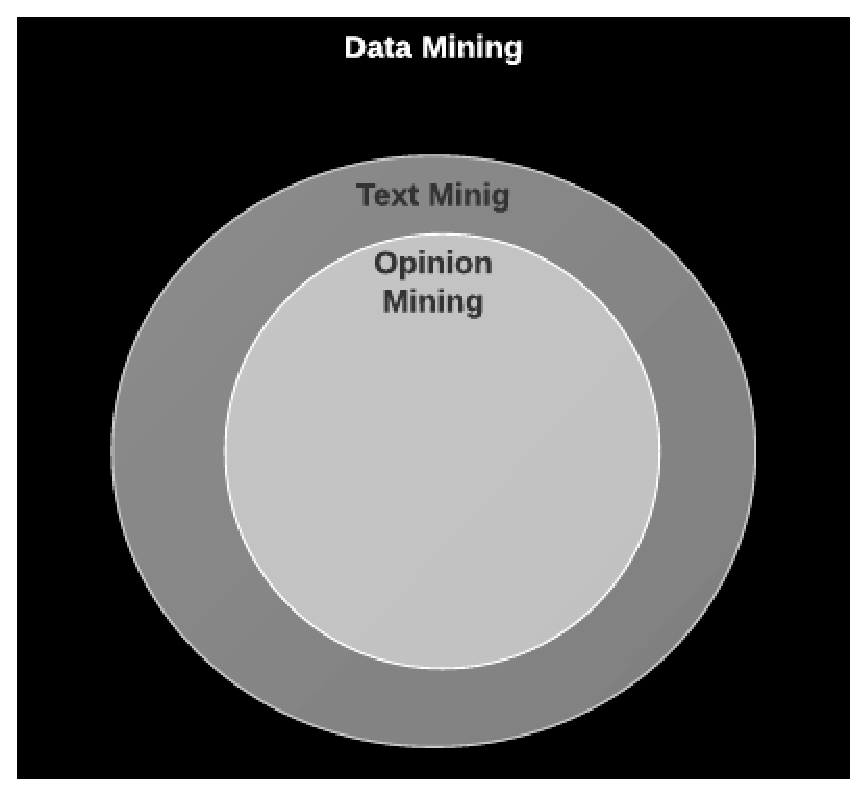
\epsfig{file=figuras/venn.eps, width=5cm}
	\caption{Diagrama de Venn - Mineração de Dados}
	\label{uni}
\end{figure}

\subsection{Sentimento}
De acordo com psicólogo Klaus R. Scherer, sentimento é um breve episódio da resposta sincronizada de todos os ou grande parte dos subsistemas orgânicos em resposta a um evento interno ou externo de grande significância\cite{scherer2001emotional}. Algumas outras definições utilizadas são:
\begin{itemize}
	\item Ato ou efeito de sentir;
	\item Aptidão para receber as impressões;
	\item Sensação, sensibilidade;
	\item Consciência íntima;
	\item Faculdade de compreender, intuição e percepção;
\end{itemize}

A mineração de opinião, também conhecida como mineração de sentimento, análise de sentimento ou extração de opinião, é um campo dentro da mineração de dados \cite{santos2014mineraccao} que tem como objetivo extrair o sentimento do texto escrito por uma pessoa, sem a interferência humana durante o processo. Porém, existe dificuldade em afirmar categoricamente o que é sentimento. 

\subsection{Desafios}

No campo de mineração de opinião, existem uma série de desafios que devem ser tidos como grandes pontos de atenção para quem deseja aplicar essa técnica de forma correta. 

\begin{itemize}
	\item Em blogs e redes sociais é comum encontrar textos com erros de ortografia ou escritos de forma informal, contendo gírias e abreviações comuns dentro da comunicação virtual;
	\item Dificuldade em discernir uma opinião ou um fato, especialmente quando existem opiniões embutidas em fatos;
	\item Os textos podem conter ironias e sarcarmos, que são especialmente difíceis de serem identificados e podem impactar os resultados;
	\item Um texto pode se referir à dois temas diferentes - política e ideologia, por exemplo - com opiniões diferentes sobre os mesmos, o que pode confundir a classificação;
\end{itemize}

\subsection{Etapas}

O processo de mineração de opinião consiste em 3 etapas: \cite{mineracaoopiniaoufsc}

\begin{itemize}
	\item Coleta de dados;
	\item Classificação;
	\item Análise dos resultados;
\end{itemize}

\subsubsection{Coleta de dados}

Nesta etapa é conduzida uma busca por opiniões nas mais diversas fontes que podem ser úteis: artigos, sites, comentários, anúncios dentre outras. Como explicado anteriormente, deve-se visar identificar se a informação coletada é uma opinião ou fato. Fatos podem ser descartados imediatamente, porém opiniões apresentadas através de fatos, podem ser úteis.

Existem diversas maneiras de coletar sistematicamente fontes para extrair e armazenar os dados que serão utilizados, dentre elas as mais famosas estão o desenvolvimento \textit{crawlers} e a utilização de APIs.

\subsubsection{Classificação}

A classificação é a alma do processo de mineração de opinião. Nesta etapa é determinada a polaridade do objeto de estudo, pretendendo determinar se o mesmo é positiva, negativa ou neutra.

Essa etapa é a principal responsável pela acurácia da análise. Por ser a etapa mais delicada do processo é onde ocorrem a maior parte dos erros. Existem diversas técnicas e ferramentas que ajudam a mitigar tais problemas que serão abordadas mais adiante, no Capítulo~\ref{cap:proposta}.

\subsubsection{Análise dos resultados}

A análise dos resultados envolve cruzar as informações de polaridade obtidas através texto com qualquer outra informação que exista sobre quem produziu aquela opinião. Desta forma, é possível, por exemplo, determinar qual gênero - masculino ou feminino - tem uma maior aceitação à um produto ou personalidade. As possibilidades para cruzar os dados e obter \textit{insights} será proporcional a quantidade de informações coletadas durante o processo.

\subsection{Aplicações práticas}

Um algoritmo capaz de extrair opiniões de um texto pode ser aplicado em diversos cenários:

\subsubsection{Pesquisa de opinião sobre um produto}

Mineração de opinião pode ser usada por uma companhia para determinar se um certo produto lançado ao mercado atingiu a aceitação prevista, como forma de entender a percepção do público e guiar estrategicamente ações de marketing e relações públicas. Ainda é possível prospectar o sentimento associado a um produto antes mesmo do seu lançamento, visando antecipar \textit{insights} que podem ser valiosos durante o seu desenvolvimento.

\subsubsection{Análise sobre pessoas públicas}

Da mesma forma, é possível utilizar a mesma técnica e direcionar as análises para uma personalidade pública. Por exemplo, é possível determinar a aceitação ou rejeição de um político durante o mandato ou período de eleições, gerando dados que podem ser decisivos na definição de suas estratégias de campanha. (REFRÊNCIA AQUI SOBRE IMPORTANCIA DE PESQUISA DE OPINIÃO NA POLÍTICA)

\subsubsection{Bolsa de valores}

Os números do mercado financeiro são uma consequência direta do sentimento que pessoas(investidores) possuem sobre uma empresa. (REFERÊNCIA SOBRE COMO MERCADO FINANCEIRO É "HUMANO" E DIRIGIDO POR EMOÇÕES) A opinião extraída de especialistas e sites de notícias podem ser usados como um dos fatores decisivos para compra e venda de ações.

\subsection{Fontes de dados}

É notório que estamos rodeados de dados dentro da Internet, porém dentro do campo de minerações de opiniões, existem algumas fontes que se destacam pela abrangência e diversidade dos dados.

\subsubsection{Mecanismos de busca}

É possível utilizar mecanismos de busca para obter opiniões sobre praticamente qualquer temática. Este método possui uma particularidade: mecanismos de busca como Google e Bing destacam certas páginas de acordo com motivos desconhecidos (RESCREVER MELHOR ISSO AQUI), o que pode influenciar os resultados obtidos. De forma geral, essa análise é apenas um reflexo do que está sendo buscado naquele momento.

Um exemplo da utilização de mecanismos de busca para mineração de opinião é o site whatdoesinternetthink.net\cite{whatdoesinternetthink}, que utiliza como base os mecanismos de busca Google e Bing para determinar a opinião sobre um tema específico ou comparar dois temas entre si.

\subsubsection{Redes sociais}

O intenso compartilhamento de informações o opiniões que vemos hoje nas redes sociais serve como uma excelente fonte de dados para a mineração de opiniões por dois motivos: diversidade e abundância. Somando-se os usuários de Facebook e Twitter por exemplo, obtemos uma amostra considerável da população mundial à disposição para pesquisas.

Para este trabalho, o Twitter foi escolhido como base para a coleta de dados, por ser uma rede social focada em opiniões de usuários e pela grande facilidade que existe em consumir os seus dados através da API pública disponibilizada pelo mesmo.

\section{Twitter}\label{sec:twitter}

Contando com uma base ativa de usuários que ultrapassa 300 milhões\cite{twittercompany2016}, o Twitter é conhecido como um \emph{microblog} fundado em março de 2006 por Jack Dorsey, Evan Williams e Biz Stone. Após 10 anos de mercado, a empresa acumula números impressionantes: 300 bilhões de mensagens já foram compartilhadas por seus usuários, que em média enviam 500 milhões de \emph{tweets}\cite{twitterstats2016} - nome pelo qual as mensagens compartilhadas no microblog ficaram conhecidas na Internet - por dia. Os usuários trocam mensagens de até 140 caracteres\cite{twittercharlimit2016} em um ambiente de rede social, que tem como objetivo dar à todos o poder de criar e compartilhar ideias e informações instantaneamente, sem barreiras\cite{twittercompany2016}. 

Dentro do Twitter, O usuário pode fazer uso de marcadores conhecidos como \emph{hashtags}\cite{waite2012paperback}, para vincular sua mensagem à um tópico específico. Apesar de simples, as \emph{hashtags} pode ser usadas das mais diversas maneiras:
\begin{itemize}
\item Agrupar comentários e pensamentos acerca de um tema
\item Estabelecer uma conexão entre dois tópicos
\item Aproximar o usuários de um conteúdo relevante com auxílio de uma busca
\end{itemize}

\subsection{Primavera Árabe}
Um dos exemplos mais recentes e impressionantes de como as redes sociais desempenharam o papel de aproximar ideologias semelhantes e encorajar debates sociais profundos foi a Primavera Árabe - onda de manifestações e protestos que tiveram início em dezembro de 2010, tendo como cenário o Norte da África e Oriente Médio. Os principais alvos foram os regimes ditatoriais e patriarcais que há muito tempo estavam no poder.\cite{howard2011opening}. Redes sociais foram amplamente utilizadas para marcar encontros, debates e manifestações, além de mostrar para o mundo o que acontecia em tempo real, através do Twitter e outras redes sociais, como o YouTube.

\begin{figure}[!h]
	\centering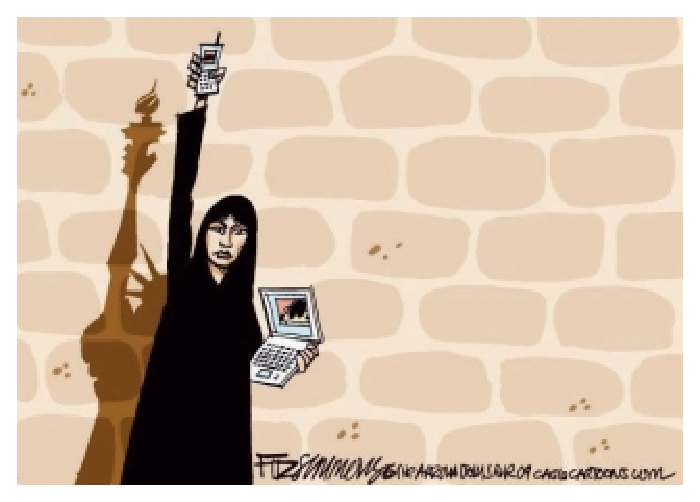
\epsfig{file=figuras/primavera_arabe_redes_sociais.eps, width=10cm}
	\caption{O celular e a internet foram as armas dos rebeldes na Primavera Árabe. Fonte: Desconhecida}
	\label{uni}
\end{figure}

\subsection{Análises de redes sociais}
Este novo cenário possibilitou que a análise de redes sociais ganhasse incrível relevância nos campos de pesquisa social e comportamental\cite{wasserman1994advances}. Ao invés de analisar comportamentos individuais, atitudes e crenças, a análise de redes sociais foca sua atenção em entidades sociais ou atores interagindo entre si e como essas interações constituem uma estrutura que pode ser estudada e analisada.

Outro ponto levantado recorrentemente quando o assunto é análise de redes sociais é o como ela pode ser útil para estudos de ordem micro ou macro. No nível \textit{micro}, as análises destinam-se a examinar díades, tríades ou outros pequenos sub-grupos. No nível \textit{macro}, o objeto de estudo são grandes redes de atores sociais.
Todos os dados obtidos durante a coleta permitem segmentar os atores sociais de diversas formas - gênero, idade, religião, posição demográfica, entre outros - possibilitando análises \textit{micro} - a nível de apenas um usuário - ou \textit{macro} - quando analisamos um conjunto de usuários. Por exemplo, os dados extraídos a partir da API do Twitter, que será abordada no Capítulo 3, nos permite entender como um usuário específico reagiu a uma \textit{hashtag}. Da mesma forma, podemos olhar um cenário mais amplo, como por exemplo, todos usuários de uma região do país. As possibilidades de análise crescem e se tornam mais ricas conforme obtemos mais informações sobre os atores no momento de suas interações sociais.

\section{API}\label{sec:api}

Por definição formal, uma API é um conjunto de rotinas estabelecidos por um software para a utilização de suas funcionalidades e acessos à seus dados por outro software que não pretende entender sobre a sua implementação, apenas seus serviços. Através dessa interface, capaz de fazer uma abstração dos dados e funcionalidades de um software, conectar-se a estes serviços se torna muito mais fácil, para ambos os lados.

Outro ponto que demonstra a importância das APIs durante o desenvolvimento de software é a interoperabilidade. Atualmente, temos o mesmo serviço sendo oferecido em diferentes plataformas, como por exemplo \textit{web}, \textit{desktop}, \textit{mobile}, entre outras. Cada plataforma possui características e implementações diferentes, porém é possível que todas as plataformas utilizem as APIs como meio único de acesso a dados e serviços, promovendo uma padronização de protocolos e funcionalidades e serviços, além de alta reusabilidade de código.

\begin{figure}[!h]
	\centering\epsfig{file=figuras/interoperabilidade_api.eps, width=10cm}
	\caption{Papel das APIs integrando dados e serviços em diferentes plataformas. Fonte: http://www.programmableweb.com/}
	\label{uni}
\end{figure}

O Twitter, nossa fonte de dados durante este trabalho, possui uma API pública que pode ser utilizada por qualquer usuário da rede social \cite{twitterapidocs}. Atualmente, é a API mais utilizada no mundo, com mais de 15 bilhões de requisições por dia, 3 vezes mais acionada do que as APIs do Google, segundo colocado no ranking.

\begin{figure}[!h]
	\centering
\epsfig{file=figuras/api_mais_usada.eps, width=10cm}
	\caption{APIs mais utilizadas do mundo Fonte: SmartFile}
	\label{uni}
\end{figure}

Para efetuar uma comunicação eficiente com quem acessa à API, é necessário implementar um protocolo de acesso aos dados. Entre eles, os mais utilizados são os protocolos REST e SOAP. O primeiro é o mais popular atualmente, segundo levantamento. (REFERÊNCIA)

\subsection{REST}
O protocolo REST foi criado em 2000 por Roy Fielding \cite{fieldingrest} durante sua dissertação de doutourado na \textit{University of California Irvine}. Por ter sido criado dentro de um ambiente universitário, o objetivo do protocolo abraça a filosofia \textit{open source}. Suas principais vantagens são:

\begin{itemize}
\item Segue a filosofia \textit{open source};
\item Fácil implementação e manutenção;
\item Separa claramente a implementação do cliente e do servidor;
\item A comunicação não é controlada por uma entidade única;
\item A informação pode ser armazenada pelo cliente previnindo múltiplas chamadas;
\item Pode retornar a informação em múltiplos formatos (JSON, XML, entre outros);
\end{itemize}

Por outro lado, o protocolo REST possui algumas limitações. Entre elas, podemos destacar:

\begin{itemize}
	\item Só funciona em cima do protocolo HTTP;
	\item Autorização e recursos de segurança devem ser implementados à parte;
\end{itemize}

Baseado nessas características, o protocolo REST é comumente utilizado para APIs de aplicações \textit{Web} e \textit{Mobile}, como por exemplo, a API do Twitter, LinkedIn e Slack. (REFERÊNCIAS)

\subsection{SOAP}
Criado em 1998 por Dave Winer et al com colaboração da Microsoft (REFERÊNCIA), o protocolo SOAP foca-se em endereçar necessidades do mercado corporativo. Como vantagem, o protocolo apresenta os seguintes aspectos:

\begin{itemize}
	\item Segue uma abordagem mais formal, corporativa;
	\item Trabalha em cima de qualquer protocolo de comunicação, até mesmo assíncrono;
	\item Recursos de autorização e segurança incorporados de forma nativa;
	\item Pode ser descrito utilizando WSDL;
\end{itemize}

Entre suas principais desvantagens, podemos listar:

\begin{itemize}
	\item Gasta-se muita banda trafegando metadados
	\item Difícil e implementação
	\item Pouco popular entre desenvolvedores \textit{Web} e \textit{Mobile}
	\item Retorna informação apenas em XML
\end{itemize}

Geralmente, o protocolo SOAP é mais utilizado em serviços financeiros, \textit{gateways} de pagamento e serviços de telecomunicações.

\section{Processamento de linguagem natural}\label{sec:pnl}

\subsection{Definição}

\ac{PNL} baseia-se em modelos computacionais capazes de executar tarefas envolvem processar informações expresas em língua natural, como por exemplo, interpretação e tradução de textos. \cite{covington1994natural}.

A pesquisa na área está voltada a três aspectos da comunicação essenciais:

\begin{itemize}
	\item fonologia: estudo dos sons;
	\item morfologia: estudo da estrutura das palavras;
	\item semântica: estudo do significado;
	\item pragmática: estudo do significado aplicado a um contexto;
\end{itemize}

Neste trabalho, focaremos apenas na PNL aplicada à area da semântica e pragmática, responsável por estudar os elementos usados durante uma comunicação para se expressar através da língua (semântica) e a diversidade que pode surgir a partir de um contexto (pragmática). É também um estudo sobre como usuários de uma língua adquirem conhecimento sobre a mesma, através da comunicação oral ou escrita e como essa língua se altera ao longo do tempo.

Um dos grandes desafios da área é modelar o processamento de uma máquina para compreender uma estrutura tão complexa como uma linguagem. Existe um teste famoso na área de computação, o Teste de Turing, que levanta a questão "As máquinas podem pensar?". O artigo fundamenta conceitos chave sobre a \ac{IA}, que serve como base para o PNL.

\subsection{Teste de Turing}

Introduzido pelo matemático britânico Alan Turing em seu artigo de 1950 "\textit{Computing Machinery and Intelligence} \cite{turing1950computing}, o Teste de Turing explora a capacidade de um computador demonstrar comportamento inteligente equivalente ou indistiguível dos seres humanos.

O teste é composto por três elementos: dois seres humanos, sendo um participante e um juiz e um computador.

O juiz conversa em linguagem natural com um outro ser humano e uma máquina através de um canal de texto, composto por um teclado e uma tela que renderiza a conversa. Todos os participantes estão em ambientes separados. O juiz deve ser capaz de distinguir a máquina do ser humano, caso contrário, a máquina é considerada bem sucedida no teste. O objetivo não é analisar se a máquina é capaz de responder corretamente e sim dizer quão próximas as respostas da máquina foram das do ser humano.  

\begin{figure}[!h]
	\centering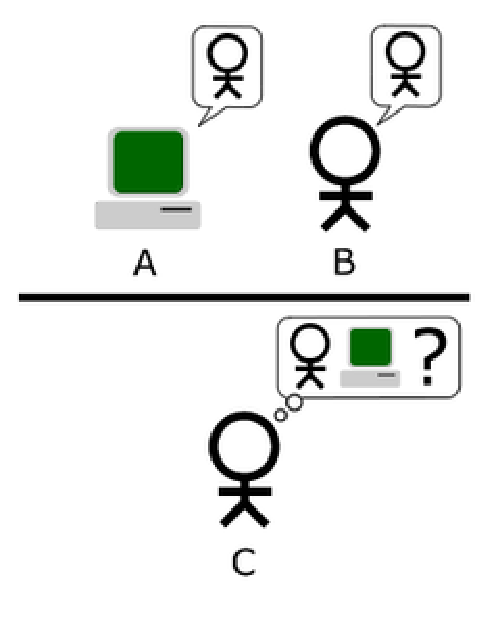
\epsfig{file=figuras/teste_turing.eps, width=10cm}
	\caption{O participante A (máquina) e o participante B (humano) se comunicam por texto com o participante C (juiz). Fonte: Wikipédia}
	\label{uni}
\end{figure}


\section{Naive Bayes (INCOMPLETO)}\label{sec:naive_bayes}
* O que é o Naive Bayes
* Demonstração matemática do algoritmo
* Uso dele em analise de sentimento/classificação


\emph{Naive Bayes} é um algoritmo probabilístico. Baseado no teorema de bayes. $$ P(A \mid B) = \frac{P(B \mid A) \, P(A)}{P(B)} $$ onde se infere qual é a probabilidade de um evento A dado um evento B. Porém nesse trabalho é utilizado o \emph{Naive Bayes} e sua diferença para o teorema de Bayes é assumir que a posição das palavras que aparecem no texto não importa, daí é acrescentado o \emph{naive}(ingênuo) ao teorema.
\\ Como visto em \cite{lucca2013implementaccao} o algoritmo computa qual a probabilidade de uma frase, denominada de documento pertencer a uma determinada classe(polaridade) \emph{P(c/d)}, a partir da probabilidade a \emph{priori} de \emph{P(c)} do documento pertencer a esta classe e da probabilidades condicionais de cada termo \emph{tk} ocorrer em um documento da mesma classe. O algoritmo tem como objetivo encontrar a melhor classe para um documento maximizando a probabilidade a\emph{posteriori} conforme a equação abaixo, onde $ n_{d} $ é o número de termos no documento \emph{d}. $$ C_{map}= argmax_{c \epsilon C}P(c|d)=argmax_{c \epsilon C}P(c)\prod 1sksn_{d}P(t_{k}/d) $$
\chapter{Proposta} \label{cap:proposta}

Como visto no Capítulo 2, existe uma corrente dentro da Mineração de Opinião que vem desenvolvendo maneiras de explorar o conteúdo digital gerado pela nossa sociedade todos os dias em redes sociais, através de técnicas utilizando Processamento de Linguagem Natural e \textit{Machine Learning}, principalmente. Com este fato surge a oportunidade de explorar novas ferramentas na
solução de problemas que envolvem pesquisas de opinião de forma geral.
Neste trabalho propõem-se um \textit{framework} que torna possível fazer pesquisas de opiniões em língua portuguesa sobre qualquer tema que seja rastreável a partir de uma \textit{hashtag} no Twitter.
Para tal é necessário que o framework criado seja capaz de:

\begin{enumerate}
	\item Coletar \textit{tweets} escritos em língua portuguesa que contenham uma determinada {hashtag};
	\item Armazenar as mensagens em uma base de dados;
	\item Classificar as mensagens de acordo com a polaridade: negativo, neutro e positivo;
	\item Extrair \textit{insights} que auxiliem a tomada de decisão a partir da massa de dados classificada;
\end{enumerate}

\section{Coleta de dados}
A plataforma do Twitter conecta aplicações e sites com seus dados através de diversos serviços. Para este trabalho, a principal fonte de dados será sua API REST, que possui uma excelente documentação disponível em \cite{twitterapidocs}. Através dela é possível acessar informações de usuários e \textit{tweets}, assim como escrever novas mensagens. Além disso, a API conta com um mecanismo de busca poderoso, que será fundamental para a coleta de dados. Os dados são entregues no formato \ac{JSON}.

\subsection{Autenticação}

Para que ter acesso à API antes é necessário possuir uma conta no Twitter e criar uma \textit{app} - através do próprio site \cite{twitterapp} - que utilizará o protocolo de autenticação OAuth\cite{oauth} para acessar os dados do Twitter se passando pelo usuário em questão. O objetivo do protocolo OAuth é permitir que uma aplicação se autentique em outra "em nome de um usuário". A aplicação pede permissão de acesso ao usuário, que possui a escolha de conceder permissão ou não. Um ponto importante: o usuário não precisa informar a sua senha para se autenticar, portanto a permissão continua vigente caso a senha do usuário se altere, o que permite que a aplicação não precise de manutenção neste caso, tornando-a mais resiliente. A autenticação por meio do OAuth necessita de três passos:

\begin{enumerate}
	\item Aplicação cliente obtém chave de autenticação;
	\item Usuário autoriza aplicação cliente na aplicação servidora;
	\item Aplicação cliente troca a chave de autenticação pela chave de acesso;
\end{enumerate}

Após o processo de criação da app, é criado um token de acesso que deve ser utilizado pelo sistema que deseja se autenticar no Twitter em nome de um usuário. Este token deve ser incorporado em cada requisição à API do Twitter para autenticar a mesma e dizer ao Twitter qual é a fonte do acesso.

\subsection{Limite de requisições}
A fim de evitar grande concentração de requisições em seus serviços, o Twitter implementa um limitador em sua API \cite{twitterrequestlimit2016}. São permitidas até 180 requisições por janela, que dura 15 minutos. Caso o limite seja ultrapassado, o serviço passa a retornar um erro na resposta, até que a "janela" de 15 minutos se renove.
A partir da versão 1.1 da API, novos cabeçalhos HTTP são retornados provendo feedback sobre os limites para requisição. Este recurso permite que o código consiga entender em que momento da janela se encontra, quantos requisições ainda podem ser feitas neste período de tempo e quanto é necessário esperar para poder fazer novas requisições. Os cabeçalhos em questão são:

\begin{itemize}
	\item X-Rate-Limit-Limit: A faixa limite para o requisição em questão;
	\item X-Rate-Limit-Remaining: O número de requisições que ainda restam para a janela de 15 minutos;
	\item X-Rate-Limit-Reset: O tempo restante dentro da janela de requisições atual, dado em segundos.
\end{itemize}

\subsection{Arquitetura}

Neste trabalho, como o objetivo é coletar \textit{tweets} postados sobre uma \textit{hashtag} em tempo real para utilizá-los como matéria-prima para análise de sentimento, é muito importante aproveitar ao máximo cada janela de requisições. Por este motivo, o sistema que coleta os dados da API do Twitter foi inspirado no modelo produtor-consumidor\cite{jeffay1993real} visando minimizar as perdas que podem acontecer em momentos de pico - como o começo ou clímax do evento, onde o volume de mensagens é maior, como veremos a frente no Capítulo 4 - e se necessário, escalar de forma simples durante os mesmos. 

\subsubsection{Produtor-consumidor}

O problema descreve dois processos, o produtor e o consumidor, que compartilham um recurso em comum usado como uma fila - um tipo particular de coleção de dados onde a primeira a entidade a entrar é a primeira a sair ou \textit{First-In-First-Out} (FIFO). A função do produtor é gerar trabalho a ser executado pelo consumidor. O volume de trabalho gerado e executado pelo sistema é controlado pela fila, que armazena as entidades ou "tarefas" a serem executadas. Essa abordagem permite que o sistema escale apenas até a sua capacidade, visto que a fila possui um tamanho fixo que caso seja ultrapassado, pode simplesmente descartar as mensagens adicionadas após este momento. Outra característica importante é a escalabilidade. Conforme os processos produtor e consumidor evoluem, surge a necessidade de aumentar a quantidade de produtores ou consumidores de forma independente.

Neste trabalho, para explorar o potencial máximo da janela de requisições foi criado um processo produtor que envia para a fila mensagens para que consumidor acesse à API do Twitter de forma que sejam feitos sempre as 180 requisições que são permitidas no intervalo de 15 minutos. Assim a responsabilidade de cada processo fica bem definida - o primeiro responde pelo volume de requisições e o segundo por realizar a requisição e entender a resposta. Para definir qual intervalo de tempo deveria ser usado para que o produtor envie mensagens à fila, foi feita uma conta simples:

$$ \frac{180}{15} = 12 \textit{ requests}_{/minuto} $$

Logo, o produtor precisa adicionar uma mensagem na fila a cada 5 segundos, para que o limite de 180 requisições seja respeitado.

\todo{Fazer diagrama do produtor-consumidor para explicar melhor}

\subsection{Busca}
Dentre os principais serviços da API do Twitter está a busca. Com ela, é possível consultar de diversas formas os principais \textit{tweets} ou mais recentes. Dentro de sua documentação, existe um guia completo de como utilizar a API  para extrair os resultados desejados \cite{twittersearchapi} das mais diversas formas. 

\subsubsection{Parâmetros adicionais}

Como abordado acima, a API possui diversos parâmetros que podem ser usados para que o usuário chegue a um conjunto de dados mais próximo da sua necessidade:

\begin{itemize}
	\item \textit{\textbf{result\_type}}: permite escolher se o resultado da busca será representado pelos \textit{tweets} mais populares (\textit{popular}) ou mais recentes (\textit{recent});
	\item \textit{\textbf{geocode}}: permite buscar por uma determinada latitude, longitude e raio, respectivamente, separando-os por vírgula. ex: geocode=-22.912214,-43.230182,1km;
	\item \textit{\textbf{lang}}: restringe os \textit{tweets} buscados a um idioma específico. ex: lang=pt;
	\item \textit{\textbf{since\_id }},  \textit{\textbf{max\_id }}, \textit{\textbf{count}} e \textit{\textbf{until}}: possibilita iterar através dos resultados quando existe um grande números de \textit{tweets} a percorrer. De acordo com a concorrência e o volume, esta tarefa pode ficar mais complicada. Uma leitura recomendada se encontra em \cite{workingwithtimelimes}.
\end{itemize}

Como o objetivo deste trabalho é coletar novos \textit{tweets} conforme eles vão sendo postados, foi necessário utilizar apenas dois parâmetros da API de busca: \textit{count} e \textit{since id}. O primeiro tem o objetivo de garantir o número máximo de registros retornados pela API e o segundo define de onde se pretende partir para buscar novos \textit{tweets}, evitando que mensagens repetidas sejam coletadas.

\url{https://api.twitter.com/1.1/search/tweets.json?q=#oscars2016&count=100&since_id=123456789}

Neste caso, a API retornará os 100 \textit{tweets} publicados desde o \textit{tweet} com identificador (\textit{id}) "123456789".

\todo{Diagrama de sequência ou atividades sobre como esta parte do código funciona}

\subsubsection{O problema com a detecção automática de idioma do Twitter}

O escopo deste trabalho determina que o objeto de estudo são apenas mensagens escritas em língua portuguesa. Como forma de obter somente \textit{tweets} escritos em língua portuguesa é preciso utilizar o parâmetro \textit{lang}, por exemplo:

\url{https://api.twitter.com/1.1/search/tweets.json?q=#oscars2016&lang=pt&result_type=recent}

Porém, realizando alguns testes na API do Twitter, foi detectado que ao submeter algum \textit{tweet}, alguma rotina dentro do próprio Twitter atribui um idioma à mensagem automaticamente. Nos testes conduzidos durante este trabalho foi identificado que em mensagens curtas - algo recorrente no Twitter - o algoritmo apresenta resultados aquém do esperado na identificação do idioma, visto que as poucas palavras contidas na mensagem podem ser comuns a mais de um idioma. Por conta disso foi decidido que o filtro de idioma não seria utilizado. Esta decisão pode mudar de acordo com o evento monitorado ou com o escopo do estudo.

\subsubsection{Escalando de forma horizontal}

Por uma questão de desenho da API de busca, cada requisição é capaz de trazer no máximo 100 \textit{tweets}, o que nos dá ao total uma carga máxima de até 1200 novos \textit{tweets} por minuto. Para as análises feitas durante este trabalho este número se mostrou mais do que suficiente. Como dito anteriormente, se fosse necessário escalar este sistema para monitorar um evento maior, seria necessário apenas obter um saldo maior de requisições junto a API do Twitter - adicionando mais tokens de usuário e criando uma espécie de "rodízio" de autenticações, por exemplo - e escalar o número de consumidores do processo de acordo com a demanda. Uma boa maneira de detectar se isso seria necessário é acompanhar quantos \textit{tweets} novos são coletados a cada requisição. Como utilizamos o \textit{id} do último \textit{tweet} capturado como referência para os novos, se a cada requisição o número de novos \textit{tweets} com grande frequência coincidir com o limite da API, temos um indício de que o volume de novas mensagens no Twitter está excedendo a capacidade do sistema de coletá-las e que o excedente está sendo perdido.

\section{Armazenamento}
A resposta da API de Busca é dada no formato JSON e cada objeto - que corresponde a cada \textit{tweet} - segue o seguinte formato e conta com diversas informações sobre o mesmo: 

\begin{lstlisting}[style=json, frame=single]
{
	"_id" : "56d388096861353c1b061fe2",
	"contributors" : null,
	"truncated" : false,
	"text" : "Leonardo DiCaprio com o #oscars eh igual a Katy Perry com o Grammy #OscarsNaTNT",
	"is_quote_status" : false,
	"in_reply_to_status_id" : null,
	"id" : 704091511902834688,
	"favorite_count" : 0,
	"source" : "<a href=\"http://twitter.com/download/android\" rel=\"nofollow\">Twitter for Android</a>",
	"created_at_datetime" : ISODate("2016-02-28T20:51:12.000Z"),
	"retweeted" : false,
	"coordinates" : null,
	"created_at_timestamp" : 1456714272.0000000000000000,
	"entities" : {
		"symbols" : [],
		"user_mentions" : [],
		"hashtags" : [{
			"indices" : [ 24, 31 ],
			"text" : "oscars"
		}, 
		{
			"indices" : [ 66, 78],
			"text" : "OscarsNaTNT"
		}],
		"urls" : []
	},
	"in_reply_to_screen_name" : null,
	"id_str" : "704091511902834688",
	"retweet_count" : 0,
	"in_reply_to_user_id" : null,
	"favorited" : false,
	"user" : {
		"follow_request_sent" : false,
		"has_extended_profile" : true,
		"profile_use_background_image" : false,
		"id" : 2786117482,
		"verified" : false,
		"profile_text_color" : "000000",
		"profile_image_url_https" : "https://pbs.twimg.com/profile_images/700450356141158404/xA-mRqp7_normal.jpg",
		"profile_sidebar_fill_color" : "000000",
		"is_translator" : false,
		"entities" : {
			"description" : {
			"urls" : []
			}
		},
		"followers_count" : 156,
		"protected" : false,
		"location" : "Um lugarzinho no fim do mundo",
		"default_profile_image" : false,
		"id_str" : "2786117482",
		"lang" : "pt",
		"utc_offset" : -28800,
		"statuses_count" : 6171,
		"description" : "Uuuumm ta estilosa!",
		"friends_count" : 192,
		"profile_background_image_url_https" : "https://abs.twimg.com/images/themes/theme1/bg.png",
		"profile_link_color" : "9266CC",
		"profile_image_url" : "http://pbs.twimg.com/profile_images/700450356141158404/xA-mRqp7_normal.jpg",
		"notifications" : false,
		"geo_enabled" : false,
		"profile_background_color" : "000000",
		"profile_banner_url" : "https://pbs.twimg.com/profile_banners/2786117482/1456444936",
		"profile_background_image_url" : "http://abs.twimg.com/images/themes/theme1/bg.png",
		"name" : "Padeira Estilosa",
		"is_translation_enabled" : false,
		"profile_background_tile" : false,
		"favourites_count" : 6095,
		"screen_name" : "naycordeir",
		"url" : null,
		"created_at" : "Fri Sep 26 18:43:47 +0000 2014",
		"contributors_enabled" : false,
		"time_zone" : "Pacific Time (US & Canada)",
		"profile_sidebar_border_color" : "000000",
		"default_profile" : false,
		"following" : false,
		"listed_count" : 1
	},
	"geo" : null,
	"in_reply_to_user_id_str" : null,
	"lang" : "pt",
	"created_at" : "Sun Feb 28 23:51:12 +0000 2016",
	"metadata" : {
		"iso_language_code" : "pt",
		"result_type" : "recent"
	},
	"in_reply_to_status_id_str" : null,
	"place" : null
}
\end{lstlisting}

Dentro desta resposta, existem diversos dados que podem ser úteis para análises em cima dos \textit{tweets} e armazená-los é extremamente valioso.

\subsection{Banco de dados orientado a documento}

Existem diversas soluções de banco de dados disponíveis no mercado. Nos últimos anos, uma delas se tornou especialmente popular\cite{bhuvan2015technical}: os bancos de dados orientado a documento. Tais bancos de dado são uma das principais categorias de bancos conhecidos NoSQL (\textit{Non Structure Query Language}) que consiste em organizar os dados de forma "não-relacional", através de documentos, gráficos, chave-valores e colunas. Bancos NoSQL são conhecidos pela facilidade de modelagem e desenvolvimento, alto desempenho de leitura e escrita, alta disponibilidade e resiliência. Isso não significa que bancos SQL são obsoletos ou piores, porém existem aplicações claras onde cada um desempenha um melhor papel. Podemos apontar algumas comparações, como por exemplo:

\begin{table}[H]
	\label{tabela-sql-nosql}
	\begin{tabular}{|m{2.5cm}|m{6cm}|m{6cm}|}
		 \hline	
		& Banco de dados relacional                                                                                                                                                                                                                            & Banco de dados NoSQL                                                                                                                                                                                                                                                                                                                \\ \hline 
		Modelagem   & O modelo relacional normaliza dados em estruturas tabulares conhecidas como tabelas, que consistem em linhas e colunas. Um schema define estritamente as tabelas, colunas, índices, relações entre tabelas e outros elementos do banco de dados.     & Bancos de dados não relacionais (NoSQL) normalmente não aplicam um schema. Geralmente, uma chave de partição é usada para recuperar valores, conjuntos de colunas ou documentos semiestruturados JSON, XML ou outros que contenham atributos de itens relacionados.                                                                  \\ \hline 
		Desempenho  & O desempenho normalmente depende do subsistema do disco. A otimização de consultas, índices e estrutura de tabela é necessária para alcançar máximo desempenho.                                                                                      & Desempenho geralmente é uma função do tamanho do cluster do hardware subjacente, da latência de rede e da aplicação que faz a chamada.  \\ \hline 
		Escala      & Mais fácil de aumentar a escala "verticalmente" com hardware mais rápido.,Outros investimentos são necessários para tabelas relacionais para abranger um sistema distribuído.                                                                        & Projetado para aumentar a escala "horizontalmente" usando clusters distribuídos de hardware de baixo custo para aumentar a transferência sem aumentar a latência.                                \\ \hline 
		APIs & As solicitações para armazenar e recuperar dados são comunicadas usando consultas compatíveis com structured query language (SQL). Essas consultas são analisadas e executadas por sistemas de gerenciamento de bancos de dados relacionais (RDBMS). & APIs baseadas em objetos permitem que desenvolvedores de aplicações armazenem e restaurem facilmente estruturas de dados na memória. As chaves de partição permitem que os aplicativos procurem pares de chave-valor, conjuntos de colunas ou documentos semiestruturados contendo objetos e atributos de aplicativos serializados. \\ \hline 
	\end{tabular}
		\caption{Comparação entre bancos SQL e NoSQL}
\end{table}

\subsection{Opções disponíveis}
O movimento de adoção de bancos \textit{NoSQL} está bastante enraizada no mundo \textit{open source}. Alguns projetos como Voldemort\cite{voldemortproject}, MongoDB\cite{mongodb}, Tokyo Cabinet\cite{tokyocabinet} e CouchDB\cite{couchdb}. Apesar de uma grande quantidade de opções \textit{open source}, o movimento ganhou muita força com a publicação de duas publicações sobre implementações proprietárias: o Google BigTable\cite{chang2008bigtable} e o Amazon Dynamo\cite{decandia2007dynamo}. Para este trabalho, a opção escolhida foi o MongoDB, altamente popular na comunidade \textit{open source} e com bastante material disponível com melhores práticas de criação, manutenção e configuração.

\subsection{Armazenando \textit{tweets}}
O objetivo deste trabalho é monitorar eventos através das \textit{hashtags}. E para cada uma delas é criada uma coleção - nome dado a um conjunto de documentos - dentro do banco de dados. O nome da coleção é dado pela \textit{hashtag} monitorada.

No momento onde o processo consumidor - responsável por fazer requisições na API e lidar com o retorno - é ligado ocorre a criação da coleção, caso a mesma não exista, e dentro dela começam a ser armazenados os \textit{tweets} retornados pela API, obedecendo ao mesmo formato enviado pelo Twitter. A flexibilidade dAntes do armazenamento no banco alguns campos a mais são adicionados, mas vamos entrar neste detalhe apenas na seção sobre Classificação.

\section{Classificação}
\begin{itemize}
	\item Aplicar técnicas de normalização no texto. As mesmas devem ser específicas para a língua portuguesa;
	\item Construir base de palavras e termos classificados utilizadas como insumo para o modelo matemático;
	\item Preparar uma massa de treino para validar o modelo matemático antes da execução;
	\item Calibragem do algoritmo
	\item Salvar infos sobre a classificação dentro do documento
\end{itemize}

\subsection{Normalização do texto}

A composição de um \textit{tweet} escrito por muitas vezes possui elementos que serão inúteis ou nocivos para o nosso algoritmo de classificação. Por conta disso, um dos primeiros desafios para tal é conduzir uma normalização nas mensagens, que serão nosso objeto de estudo.


\subsection{Construção da base de palavras e termos}
A construção da base de dados foi feita com o intuito de melhor expressar um sentimento de uma palavra ou texto, para a utilização do algoritmo. Para isso a base foi dividida em dois arquivos, positivos e negativos. Além dessa divisão foi utilizada outas bases criadas como: Re-li(referencia), SentiLex-PT \cite{marioj.silvapaulacarvalholuissarmento2012}, base da puc \cite{freitas2013construccao}, emoticons \cite{alexanderhogenboomdaniellabalflaviusfrasincarmalissabalfranciskadejonguzaykaymak}. Todas usando a língua portuguesa ou um linguajar universal, no caso dos emoticons e já estarem polarizadas. Essas bases têm em comum é serem feitas apenas de palavras, então ficou-se a dúvida de como a classificação funcionaria posteriormente quando aplicadas a um texto que as palavras podem não estar no mesmo contexto. Ex: "O flamengo jogou muito mal, mas fico feliz pela vitória", onde tem a palavra mal que já dá um tom negativo a frase , porém ao terminar de ler a frase encontrasse as palavras feliz e vitória que tem um contexto positivo.
Com essas bases já citadas foi compreendida a necessidade de uma base mais específica para o linguajar utilizado na internet, constituído de  
gírias, abreviação e até erros de português, para isso foi criada uma base utilizando dados pegos do twitter a partir da marcação hashtagoscar2016.


\subsection{Massa de treino}

\subsection{Massa de teste}

\subsection{Algoritmo}



\chapter{Resultados e análises}\label{cap:resultados}

Nesta seção será apresentada os resultados obtidos e os processos necessários para a obtenção dos mesmos. Como visto no Capitulo 4 uma das fases necessárias para a Análise de Sentimento é a classificação de polaridade dos \textit{tweets}. Durante a classificação, que era o resultado da execução do Naive Bayes, foram utilizadas diversas formas de execução que serão apresentadas abaixo

\section{Cenários e parâmetros de teste}\label{sec:cenarios}
Durante a execução dos testes para a análise de resultados o ambiente utilizado foi:
\begin{itemize}
	\item Sistema operacional: Linux Ubuntu
	\item Processador: Core i7
	\item Memória: 8GB
	\item Quantidade de \textit{tweets}: 141798
\end{itemize}


\section{Experimentos realizados e resultados}\label{sec:resultados}
O primeiro teste realizado para a classificação da base obteve o seguinte resultado:
\todo{Trazer tabela  1 pra ca}
\begin{table}[]
	\caption{1º teste}
	\label{teste-1}
	\resizebox{\textwidth}{!}{%
		\begin{tabular}{|l|l|r}
			\hline
			\multicolumn{3}{|c|}{1º Teste} \\ \hline
			\multicolumn{2}{|l|}{Bases usadas} & \multicolumn{1}{r|}{Tecnicas usadas} \\ \hline
			\multicolumn{2}{|c|}{Sentilex} & \multicolumn{1}{c|}{Stopwords} \\
			\multicolumn{2}{|c|}{PUC} & \multicolumn{1}{c|}{Stemming} \\ \cline{3-3} 
			\multicolumn{2}{|c|}{ReLi} &  \\ \hline
			\multicolumn{3}{|c|}{Resultado} \\ \hline
			\multicolumn{2}{|l|}{Positivo} & \multicolumn{1}{r|}{17350} \\ \hline
			\multicolumn{2}{|l|}{Negativo} & \multicolumn{1}{r|}{15517} \\ \hline
			\multicolumn{2}{|l|}{Neutro} & \multicolumn{1}{r|}{108931} \\ \hline
			\multicolumn{2}{|l|}{Tempo} & \multicolumn{1}{r|}{311.673 segundos} \\ \hline
		\end{tabular}%
	}
\end{table}

Analisando a tabela \ref{teste-1} é visto quais as bases utilizadas, nesse caso, Reli , PUC e Sentilex, as técnicas utilizadas nesse teste, \textit{Stopwords} e \textit{Stemming}, e o resultado que de 141798 \textit{tweets}, 17350 foram positivos, 15517 negativos e 108931 neutros, levando 311.673 segundos para executar o teste.
\todo{Adicionar imagem}

Observando os resultados, é visto que a quantidade de \textit{tweets} neutros é maior que a dos outros, com isso foi que havia a necessidade de diminuir a quantidade de neutros. Mudanças no cenário de testes para conseguir essa diminuição. 
\todo{Tabela 2 aqui}

\begin{table}[]
	\caption{2º teste}
	\label{teste-2}
	\resizebox{\textwidth}{!}{%
		\begin{tabular}{|l|l|r}
			\hline
			\multicolumn{3}{|c|}{2º Teste} \\ \hline
			\multicolumn{2}{|l|}{Bases usadas} & \multicolumn{1}{r|}{Tecnicas usadas} \\ \hline
			\multicolumn{2}{|c|}{Sentilex-Stem} & \multicolumn{1}{c|}{Stopwords-Stem} \\
			\multicolumn{2}{|c|}{PUC-Stem} & \multicolumn{1}{c|}{Stemming} \\ \cline{3-3} 
			\multicolumn{2}{|c|}{ReLi} &  \\ \hline
			\multicolumn{3}{|c|}{Resultado} \\ \hline
			\multicolumn{2}{|l|}{Positivo} & \multicolumn{1}{r|}{49263} \\ \hline
			\multicolumn{2}{|l|}{Negativo} & \multicolumn{1}{r|}{35079} \\ \hline
			\multicolumn{2}{|l|}{Neutro} & \multicolumn{1}{r|}{57456} \\ \hline
			\multicolumn{2}{|l|}{Tempo} & \multicolumn{1}{r|}{397.48 segundos} \\ \hline
		\end{tabular}%
	}
\end{table}

No 2º teste visto na tabela \ref{teste-2} é visto que a quantidade de neutro diminuiu consideravelmente, apenas aplicando a técnica de \textit{stemming} nas bases de palavras
\todo{grafico 2}


Ainda buscando a diminuição de neutros foi criada uma base de palavras mas próxima do domínio que esse trabalho propõe que é o Oscar2016, essa base contem palavras relevantes a esse evento, gerando o seguinte resultado.
\todo{colocar tabela 3 aqui}

\begin{table}[]
	\caption{3º teste}
	\label{teste-3}
	\resizebox{\textwidth}{!}{%
		\begin{tabular}{|l|l|r|}
			\hline
			\multicolumn{3}{|c|}{3º Teste} \\ \hline
			\multicolumn{2}{|l|}{Bases usadas} & Técnicas usadas \\ \hline
			\multicolumn{2}{|c|}{Oscar2016} & \multicolumn{1}{c|}{\textit{Stopwords}} \\ \hline
			\multicolumn{3}{|c|}{Resultado} \\ \hline
			\multicolumn{2}{|l|}{Positivo} & 47450 \\ \hline
			\multicolumn{2}{|l|}{Negativo} & 7210 \\ \hline
			\multicolumn{2}{|l|}{Neutro} & 87138 \\ \hline
			\multicolumn{2}{|l|}{Tempo} & 709,126 segundos \\ \hline
		\end{tabular}%
	}
\end{table}

Analisando a tabela \ref{teste-3} é visto que apenas uma base mais especializada no domínio não consegue diminuir a quantidade de neutros e ainda aumenta o tempo para a execução dos testes.
\todo{grafico 3}


No 4º teste foi adicionada o base criada, Oscar2016, com as bases genéricas, gerando o seguinte resultado:
\begin{table}[]
	\caption{4º teste}
	\label{teste-4}
	\resizebox{\textwidth}{!}{%
		\begin{tabular}{|c|l|r}
			\hline
			\multicolumn{3}{|c|}{4º Teste} \\ \hline
			\multicolumn{2}{|l|}{Bases usadas} & \multicolumn{1}{r|}{Técnicas usadas} \\ \hline
			\multicolumn{2}{|c|}{Oscar2016} & \multicolumn{1}{c|}{Stopwords} \\
			\multicolumn{2}{|c|}{SentiLex} & \multicolumn{1}{c|}{Stemming} \\ \cline{3-3} 
			\multicolumn{2}{|c|}{PUC} & \multicolumn{1}{c}{} \\
			\multicolumn{2}{|c|}{ReLi} & \multicolumn{1}{c}{} \\ \hline
			\multicolumn{3}{|c|}{Resultado} \\ \hline
			\multicolumn{2}{|l|}{Positivo} & \multicolumn{1}{r|}{69070} \\ \hline
			\multicolumn{2}{|l|}{Negativo} & \multicolumn{1}{r|}{33461} \\ \hline
			\multicolumn{2}{|l|}{Neutro} & \multicolumn{1}{r|}{39267} \\ \hline
			\multicolumn{2}{|l|}{Tempo} & \multicolumn{1}{r|}{650.97 segundos} \\ \hline
		\end{tabular}%
	}
\end{table}

Analisando a tabela \ref{teste-4} é visto que nesse teste foi obtida a maior diminuição de neutros, mas com um tempo de processamento um pouco maior.
\todo{Adicionar grafico 4}

Segue abaixo um comparativo dos testes.

\begin{table}[]
	\caption{Comparando testes}
	\label{teste-comp}
	\resizebox{\textwidth}{!}{%
		\begin{tabular}{l|l|c|l|l|}
			\cline{2-5}
			\multicolumn{1}{c|}{} & \multicolumn{1}{c|}{Teste 1} & Teste 2 & \multicolumn{1}{c|}{Teste 3} & \multicolumn{1}{c|}{Teste 4} \\ \hline
			\multicolumn{1}{|l|}{Positivo} & 15517 & \multicolumn{1}{r|}{49263} & 47450 & 69070 \\ \hline
			\multicolumn{1}{|l|}{Negativo} & 17350 & 35079 & 7210 & 33461 \\ \hline
			\multicolumn{1}{|l|}{Neutro} & 108931 & \multicolumn{1}{l|}{57456} & 87138 & 39267 \\ \hline
			\multicolumn{1}{|l|}{Tempo (s)} & \multicolumn{1}{c|}{311.673} & 397.48 & 709.129 & 650.97 \\ \hline
		\end{tabular}%
	}
\end{table}

\chapter{Conclusão} \label{cap:conclusao}

Este trabalho identificou e abordou a importância que a mineração de opinião possui nos dias atuais, além das oportunidades que este novo campo de estudo abre com a sua descoberta: tanto na área acadêmica quanto para exploração comercial e estratégica e assim como propôs, desenvolveu uma solução capaz de extrair mensagens escritas em língua portuguesa de uma \textit{hashtag} do Twitter e classificá-las em positivas, neutras ou negativas, tornando possível fazer análises de mineração de opinião que são capazes de interpretar como um universo de usuários se sente em relação a temática estudada. Sem dúvida, o grande desafio foi mostrar que é viável aplicar uma solução de mineração de opinião mesmo com a complexidade da língua portuguesa.
Com base no que foi apresentado, a proposta cumpriu os seguintes objetivos levantados:

\begin{itemize}
	\item Utilização do Twitter como plataforma de dados;
	\item Construção um processo escalável capaz de extrair mensagens de uma \textit{hashtag} do Twitter;
	\item Utilização bases de palavras classificadas disponíveis na literatura sobre o tema;
	\item Aplicação de técnicas de normalização de texto visando um maior desempenho ao classificar;
	\item Implementação do algoritmo de \textit{Naive Bayes} para classificar as mensagens em positivas, neutras ou negativas;
	\item Conduzir a classificação em mensagens que foram escritas em língua portuguesa;
	\item Aplicação do conhecimento adquirido durante este trabalho em um estudo de caso utilizando a cerimônia do Oscars 2016;
	\item Demonstração dos cenários de teste e seus impactos no resultado final;
	\item Análise dos resultados obtidos atraves de gráficos que permitem interpretar os sentimentos dos usuários antes, durante e depois do evento, sob diversas perspectivas.
\end{itemize}

A análise dos resultados mostrou que por existir uma ansiedade muito grande vinculada aos instantes que antecedem o evento existe uma grande concentração de sentimentos positivos atrelados a este momento. Outro fato que ficou evidente é que os momentos mais populares do evento, como o anúncio das categorias mais aguardadas como: melhor ator, melhor atriz e melhor filme são as mais esperadas e com a confirmação da vitória dos favoritos, houve um pico de mensagens positivas por volta do horário do anúncio dos vencedores destas categorias. Outros dois momentos chamaram atenção pela carga de sentimentos negativos: o show de David Grohl em homenagem aos falecidos no mundo do cinema em 2015 onde a sensação de luto ficou evidente e a apresentação de Lady Gaga, onde o tema do filme que a música  faz parte da trilha sonora aborda estupros em faculdades americanas, tema que desperta bastante tristeza nas pessoas que sofreram este tipo de trauma ou que empatizam de alguma forma com as vítimas deste crime.


\section{Trabalhos Futuros}\label{sec:8_trabfut}

Como visto neste trabalho, o algoritmo utilizado para gerar os resultados das classificações a fim de realizar a análise de sentimento foi o \textit{Naive Bayes}. Para trabalhos futuros pode-se utilizar outros algoritmos como: Árvore de Decisão, Regressão Logística, \textit{Maximum Entropy Model}. Podendo ser usados somente o próprio algoritmo ou realizando um trabalho comparativo entre eles, descobrindo qual algoritmo gera melhores resultados.

Outro método que pode ser utilizado é a aplicação de \textit{n-grams}, para averiguar o melhor desempenho do modelo. Com isso poderia-se realizar testes de acurácia, que não foi o enfoque deste trabalho. Pode-se também utilizar outras fontes de dados, não só o Twitter, como: Facebook, fórums, comentários de sites, entre outros. Mais um fator relevante são as bases, que nesse trabalho foram utilizadas três bases genéricas e uma pequena base personalizada, então como trabalho futuro propõem-se utilizar apenas bases personalizadas e referentes ao domínio.

Durante as pesquisas para esse trabalho foi encontrado um \textit{toolkit}  para a técnica de \textit{word embedding}, conhecido como \textit{word2vec}, criado em 2013 por uma equipe do Google. Esse tipo de técnica se baseia em redes neurais, que difere do algoritmo probabilístico utilizado nesse trabalho. Sendo essa uma outra proposta pra trabalhos futuros.

Entre os testes realizados no capítulo \ref{cap:resultados} foi presenciado um fator instigante. A duração dos testes,  que podem ser encontrados no apêndice \ref{teste_tempo},  foi notado um crescimento anômalo, entretanto não foi discutido a causa de tal crescimento, então é proposto um estudo onde se discute tal anomalia. 

Por fim, pretende-se fazer o máximo para desenvolver o  processamento de linguagem natural para a língua portuguesa, onde técnicas e métodos serão comparadas visando o melhor desempenho com uma análise mais profunda e a automação da inteligência artificial para o aproveitamento desse campo para o ser humano em suas tomadas de decisão. 



% --- -----------------------------------------------------------------
% --- Referencias Bibliograficas. (Obrigatorio)
% --- -----------------------------------------------------------------
\cleardoublepage
%\bibliographystyle{acm-2} 
%\bibliographystyle{abnt-num} % abbrv - abnt-num
\inputencoding{latin1}
\bibliographystyle{IEEEtran}
%\bibliographystyle{uff-ic}
\bibliography{referencia} % arquivo fonte com a bibliografia
%\bibliography{articles,books,standards,websites} % arquivo fonte com a bibliografia


%\addcontentsline{toc}{part}{Index}
%\printindex
\label{LastPage}
\end{document}